\usetikzlibrary{calc}
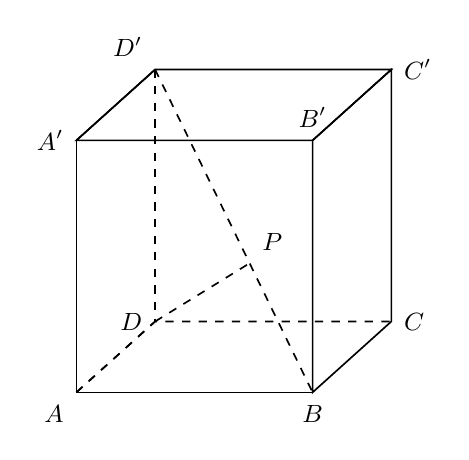
\begin{tikzpicture}[line width=.6pt, font=\small]
\coordinate (A) at (0,0);
\coordinate (B) at (3,0);
\coordinate (C) at (4,0.9);
\coordinate (D) at (1,0.9);
\coordinate (Ap) at (0,3.2);
\coordinate (Bp) at (3,3.2);
\coordinate (Cp) at (4,4.1);
\coordinate (Dpp) at (1,4.1);
\coordinate (P) at (2.2,1.64);
% front face
\draw (A)--(B)--(Bp)--(Ap)--cycle;
% top face
\draw (Ap)--(Bp)--(Cp)--(Dpp)--cycle;
\draw (Ap)--(Dpp);
% right face
\draw (B)--(Bp)--(Cp)--(C)--cycle;
% hidden bottom
\draw[dashed] (A)--(D)--(C);
% hidden vertical + body diagonal + DP
\draw[dashed] (Dpp)--(D);
\draw[dashed] (Dpp)--(B);
\draw[dashed] (D)--(P);
\draw[dashed] (A)--(D);
% labels
\node[below left=1pt] at (A) {$A$};
\node[below=1pt] at (B) {$B$};
\node[right=1pt] at (C) {$C$};
\node[left=1pt] at (D) {$D$};
\node[left=1pt] at (Ap) {$A'$};
\node[above=1pt] at (Bp) {$B'$};
\node[right=1pt] at (Cp) {$C'$};
\node[above left=1pt] at (Dpp) {$D'$};
\node[above right=1pt] at (P) {$P$};
\end{tikzpicture}
